\documentclass[a4paper, 12pt]{article}

\usepackage{graphicx}
\usepackage{amsmath}
\usepackage[a4paper,width=150mm,top=20mm,bottom=20mm,left=30mm,right=20mm]{geometry}
\usepackage{amsfonts}
\usepackage{dsfont}


\newcommand{\sout}[1][T]{|S^{out}_{#1}|}
\newcommand{\sint}[1][T]{|S^{in}_{#1}|}
\newcommand{\pop}{|\mathcal{P}|}


\begin{document}

\section{Likelihood}
\begin{itemize}
    \item $S_t$: the $t$-th sample.
    \item $n_t := |S_t|$: sample size at each sample draw. Depending on the sampling scheme, it is possible for $n_t$ to be random. For simplicity, assume that $n_t = n$ is fixed.
    \item $S_T^{in} = \bigcup \limits_{t=1}^{T} S_t$: set of sampled individuals up to and including $T$-th sample.
    \item $S_T^{out}$: set of individuals that has not been sampled after $T$ sample draws. ($S_T^{out} \cap S_T^{in} = \emptyset$).
    \item $\mathcal{P} = S_T^{in} \cup S_T^{out}$: the entire population.
    \item $d_{i(T)}$: number of samples that contained individual $i$:
    \begin{equation*}
        d_{i(T)} = \sum_{t=1}^T \mathds{1}\{i \in S_t \}
    \end{equation*}
\end{itemize}
Assuming that samples are drawn independently:
\begin{equation*}
    \mathbb{E}[d_{i(T)}] = \sum_{t = 1}^T \pi_i = T\pi_i
\end{equation*}
where $\pi_i$ denotes inclusion probability of $i$. This suggests estimating $\pi_i$ by
\begin{equation} \label{eq:1}
    \hat{\pi}_i = \frac{d_{i(T)}}{T} \quad \text{or} \quad \hat{\pi}_i = \frac{1 + d_{i(T)}}{1 + T}
\end{equation}
where the latter comes from enforcing the probabilities to be non-zero. Note that in this case $\hat{\pi_i} = \frac{1}{1 + T} \forall i \in S_T^{out}$.
\subsection{Homogenous inclusion probabilities}
Let $\pi_i = \frac{n}{\pop}$ $\forall i = 1, \dots, \pop$. Then the inclusion frequencies follow a binomial distribution.
\begin{equation*}
d_{i(T)} \overset{i.i.d.}{\sim} Bin(T, \frac{n}{\pop})
\end{equation*}
Note that we do not observe $d_{i(T)} = 0$, but only $d_{i(T)} > 0$. Truncating the distribution at 0 yields
\begin{align*}
\mathbb{P}(d_{i(T)} = k|d_{i(T)} > 0) &= \frac{\mathbb{P}(d_{i(T)} = k)}{1 - \mathbb{P}(d_{i(T)} = 0)} = \frac{\binom{T}{k} (\frac{n}{\pop})^k (\frac{\pop - n}{\pop})^{T - k}}{1 - (\frac{\pop - n}{\pop})^T}\\
&= \binom{T}{k} \frac{n^k (\pop - n)^{T-k}}{\pop^{T} - (\pop - n)^T} = \binom{T}{k} \frac{n^k (\sint + \sout - n)^{T-k}}{(\sint + \sout)^{T} - (\sint + \sout - n)^T}
\end{align*}
This leads to the joint likelihood
\begin{align*}
L(\sout) &:= L(\sout; T, d_{i(T)} = k_i \forall i \in S_T^{in}) \\
&= \prod_{i \in S_T^{in}} \binom{T}{k_i} \frac{n^{k_i} (\sint + \sout - n)^{T-k_i}}{(\sint + \sout)^{T} - (\sint + \sout - n)^T} \\
&\propto \prod_{i \in S_T^{in}} \frac{(\sint + \sout - n)^{T-k_i}}{(\sint + \sout)^{T} - (\sint + \sout - n)^T} \\
&= [(\sint + \sout)^{T} - (\sint + \sout - n)^T]^{-\sint} (\sint + \sout - n)^{T(\sint  - n)}
\end{align*}
since $\sum_{i \in S_T^{in}} k_i = nT$ for fixed $n$. Taking logarithm of the likelihood leads to
\begin{align}
l(\sout) &:= \log L(\sout) \nonumber \\
&= const - \sint \log[(\sint + \sout)^{T} - (\sint + \sout - n)^T]\nonumber \\ 
&+ T(\sint  - n) \log (\sint + \sout - n)
\end{align}
The derivative with respect to $\sout$ is
\begin{align}
\frac{d}{d\sout}l(\sout) =& -\sint T \frac{(\sint + \sout)^{T-1} - (\sint + \sout - n)^{T-1}}{(\sint + \sout)^{T} - (\sint + \sout - n)^T} \nonumber \\
&+ \frac{T(\sint  - n)}{\sout + \sint - n}
\end{align}
% Setting the derivative to zero, the first-order condition can be written as
% \begin{equation*}
% \left( \frac{\sout + \sint - n}{\sout + \sint} \right)^T - \frac{\sint T}{\sum_{i \in S_T^{in}} k_i} \left( \frac{\sout + \sint - n}{\sout + \sint} - 1 \right) - 1 \overset{!}{=} 0
% \end{equation*}
\subsubsection{Classical capture-recapture}
Setting $T = 2$ results in the following log-likelihood:
\begin{align*}
l(\sout) &= const - \sint \log[(\sint + \sout)^{2} - (\sint + \sout - n)^2] \\ 
&+ 2(\sint  - n) \log (\sint + \sout - n)
\end{align*}
The first-order condition is
\begin{equation*}
\frac{d}{d\sout}l(\sout) = -\frac{2\sint n}{(\sint + \sout)^{2} - (\sint + \sout - n)^2} + \frac{2(\sint  - n)}{\sout + \sint - n} \overset{!}{=} 0
\end{equation*}
Then, the maximum likelihood estimator of $\sout$ can be expressed as
\begin{equation}
\widehat{\sout}_{ML} = \frac{(n - \sint[2])(\sint[2] - n)}{\sint[2] - 2n}
\end{equation}
\subsubsection{One draw}
If $T = 1$, then $\sint = \sum_{i \in S_T^{in}} k_i = n$. The log-likelihood becomes
\begin{equation*}
l(\sout) = const - \sint \log(\sint) =: const
\end{equation*}
\subsection{Heterogenous inclusion probabilities}
Consider the problem from the Bayesian perspective. Assume Beta prior for inclusion probabilities:
\begin{equation*}
    \pi_i \sim Be(\alpha, \beta)
\end{equation*}
Then
\begin{equation*}
    \mathbb{E}[\sum_{i \in \mathcal{P}} \pi_i] = \sum_{i \in \mathcal{P}} \frac{\alpha}{\alpha + \beta} = |\mathcal{P}| \frac{\alpha}{\alpha + \beta} = (|S_T^{out}| + |S_T^{in}|) \frac{\alpha}{\alpha + \beta}
\end{equation*}
\begin{equation} \label{eq:2}
    \mathbb{E}[\sum_{i \in \mathcal{P}} \pi_i] = \mathbb{E}[n_t]
    \Leftrightarrow (|S_T^{out}| + |S_T^{in}|) \frac{\alpha}{\alpha + \beta} = n
\end{equation}
(in case of random $n_t$, we can estimate $\mathbb{E}[n_t]$ by $T^{-1} \sum_{t=1}^T n_t$).

\noindent Condition \eqref{eq:2} will be the constraint for our model.

\noindent The likelihood would be
\begin{equation*}
    d_{i(T)} |\pi_i \sim Bin(T, \pi)
\end{equation*}
Then the posterior distribution is
\begin{align*}
    f(\pi_i | d_{i(T)} = k) &= \frac{\mathbb{P}(d_{i(T)} = k | \pi_i) f(\pi_i)}{\mathbb{P}(d_{i(T)} = k)} \\
    &\propto \pi_i^k(1 - \pi_i)^{T - k}\pi_i^{\alpha - 1}(1 - \pi_i)^{\beta - 1}\\
    &= \pi_i^{\alpha + k - 1}(1 - \pi_i)^{\beta + T - k - 1}\\
    &\Rightarrow \pi_i | d_{i(T)} = k \sim Be(\alpha + k, \beta + T - k)\\
    &\Rightarrow \mathbb{E}[\pi_i|d_{i(T)} = k] = \frac{\alpha + k}{\alpha + \beta + T}
\end{align*}
The marginal likelihood is:
\begin{align*}
    \mathbb{P}(d_{i(T)} = k) &= \int_0^1 f(\pi_i, d_{i(T)})d\pi_i = \int_0^1 \mathbb{P}(d_{i(T)} = k | \pi_i)f(\pi_i)d\pi_i\\
    &= \binom{T}{k} \frac{\mathrm{B}(\alpha + k, \beta + T - k)}{\mathrm{B}(\alpha, \beta)}
\end{align*}
Since we never observe $d_{i(T)} = 0$, the observed frequences $d_{i(T)} > 0$ for $i \in S_{T}^{in}$ follow a truncated distribution:
\begin{align*}
\mathbb{P}(d_{i(T)} = k | d_{i(T)} > 0) &= 
\begin{cases}
    \frac{\mathbb{P}(d_{i(T)} = k)}{1 - \mathbb{P}(d_{i(T)} = 0)},& \text{if } k > 0 \\
    0, & \text{otherwise}
\end{cases}\\
&=
\begin{cases}
    \binom{T}{k} \frac{\mathrm{B}(\alpha + k, \beta + T - k)}{\mathrm{B}(\alpha, \beta) - \mathrm{B}(\alpha, \beta + T)},& \text{if } k > 0 \\
    0, & \text{otherwise}
\end{cases}
\end{align*}
Following empirical Bayes approach, maximise the marginal likelihood to obtain hyperparameters $\alpha$ and $\beta$.
\begin{align} \label{eq:3}
    L(\alpha, \beta) &:= L(\alpha, \beta; T, d_{i(T)} = k_i \forall i \in S_T^{in}) \nonumber \\
    &\overset{indep}{=} \prod_{i \in S_T^{in}} \binom{T}{k_i} \frac{\Gamma(\alpha + k_i)\Gamma(\beta + T - k_i)}{\Gamma(\alpha + \beta + T)} \cdot \frac{1}{\frac{\Gamma(\alpha)\Gamma(\beta)}{\Gamma(\alpha + \beta)} - \frac{\Gamma(\alpha)\Gamma(\beta + T)}{\Gamma(\alpha + \beta + T)}} \nonumber \\
    &= \prod_{i \in S_T^{in}} \binom{T}{k_i} \frac{\Gamma(\alpha + k_i)\Gamma(\beta + T - k_i)\Gamma(\alpha + \beta)}{\Gamma(\alpha)\Gamma(\beta)\Gamma(\alpha + \beta + T) - \Gamma(\alpha)\Gamma(\beta + T)\Gamma(\alpha + \beta)} \nonumber \\
\end{align}
Using the recursive formula of gamma function $\Gamma(x) = (x - 1)\Gamma(x - 1)$ and the fact that $T, k_i \in \mathbb{N}_0 := \mathbb{N} \cup \{0\}$ allows us to rewrite the marginal likelihood as:
\begin{align*}
    L(\alpha, \beta) &\propto \prod_{i \in S_T^{in}} \frac{\Gamma(\alpha) \Gamma(\beta) \Gamma(\alpha + \beta)}{\Gamma(\alpha)\Gamma(\beta)\Gamma(\alpha + \beta)}\\
    &\times \frac{\prod_{j=1}^{k_i} (\alpha + k_i - j)\prod_{j=1}^{T - k_i} (\beta + T - k_i - j)}{\prod_{j=1}^T(\alpha + \beta + T - j) - \prod_{j=1}^T (\beta + T - j)} \\
    &= \prod_{i \in S_T^{in}} \frac{\prod_{j=1}^{k_i} (\alpha + k_i - j)\prod_{j=1}^{T - k_i} (\beta + T - k_i - j)}{\prod_{j=1}^T(\alpha + \beta + T - j) - \prod_{j=1}^T (\beta + T - j)} 
\end{align*}
The parameters $\alpha$ and $\beta$ must satisfy \eqref{eq:2}, so equation \eqref{eq:3} is to be maximised subject to the constraint. Note that \eqref{eq:2} can be viewed as enforcing our prior to be centered at $\frac{n}{\pop}$, since 
\begin{equation*}
(|S_T^{out}| + |S_T^{in}|) \frac{\alpha}{\alpha + \beta} = n \Leftrightarrow \frac{\alpha}{\alpha + \beta} = \mathbb{E}[\pi_i] = \frac{n}{(|S_T^{out}| + |S_T^{in}|)}
\end{equation*}
Intuitively, this means that, under the constraint, the hyperparameters will determine only the variance of the prior.

The optimisation problem can be simplified by solving the constraint for $\beta$ and plugging into the objective function:
\begin{align*}
    \max_{\alpha, \beta} L(\alpha, \beta) &\quad \text{s.t.} \quad |\mathcal{P}|\frac{\alpha}{\alpha + \beta} = n \\
    &\Leftrightarrow \beta = \left(\frac{|\mathcal{P}|}{n} - 1 \right)\alpha := q\alpha\\
    \Rightarrow \max_{\alpha, q} L(\alpha, q) &
\end{align*}
More explicitly,
\begin{align*}
    \max_{\alpha, \beta} L(\alpha, \beta) &\quad \text{s.t.} \quad (\sint + \sout)\frac{\alpha}{\alpha + \beta} = n \\
    &\Leftrightarrow \beta = n^{-1}\alpha\sint + n^{-1}\alpha\sout - \alpha\\
    \Rightarrow \max_{\alpha, \sout} L(\alpha, \sout) &
\end{align*}
\subsubsection{Variant 1}
\begin{align*}
    L(\alpha, q) &\propto \prod_{i \in S_T^{in}} \frac{\prod_{j=1}^{k_i} (\alpha + k_i - j)\prod_{j=1}^{T - k_i} (q\alpha + T - k_i - j)}{\prod_{j=1}^T(\alpha + q\alpha + T - j) - \prod_{j=1}^T (q\alpha + T - j)} \\
\end{align*}
\begin{align} \label{eq:4}
    l(\alpha, q) &:= \log L(\alpha, q) \nonumber \\
    &= const - |S_T^{in}|\log\left[\prod_{j=1}^T(\alpha + q\alpha + T - j) - \prod_{j=1}^T (q\alpha + T - j)\right] \nonumber \\
    &+ \sum_{i \in S_T^{in}} \sum_{j = 1}^{k_i} \log(\alpha + k_i - j) + \sum_{j = 1}^{T - k_i} \log(q\alpha + T - k_i - j) \nonumber \\
\end{align}
Derivatives:
\begin{align} \label{eq:5}
    \frac{\partial l(\alpha, q)}{\partial \alpha} =& -\sint \frac{\sum_{j = 1}^{T} (1 + q) \prod_{1 \leq m \neq j \leq T} (\alpha + q\alpha + T - m) - \sum_{j = 1}^{T} q \prod_{1 \leq m \neq j \leq T} (q\alpha + T - m)}{\prod_{j = 1}^{T} (\alpha + q\alpha + T - j) - \prod_{j=1}^T (q\alpha + T - j)}\nonumber \\
    &+ \sum_{i \in S_T^{in}} \sum_{j = 1}^{k_i} (\alpha + k_i - j)^{-1} + q\sum_{j = 1}^{T - k_i} (q\alpha + T - k_i - j)^{-1} \nonumber \\
    =& -(1 + q)\sint \frac{ \prod_{j = 1}^{T} (\alpha + q\alpha + T - j) \sum_{j = 1}^{T} (\alpha + q\alpha + T - j)^{-1} }{\prod_{j = 1}^{T} (\alpha + q\alpha + T - j) - \prod_{j=1}^T (q\alpha + T - j)} \nonumber \\
    &+ q|S_T^{in}| \frac{\prod_{j = 1}^{T} (q\alpha + T - j) \sum_{j = 1}^{T} (q\alpha + T - j)^{-1}  }{ \prod_{j = 1}^{T} (\alpha + q\alpha + T - j) - \prod_{j=1}^T (q\alpha + T - j)} \nonumber \\
    &+ \sum_{i \in S_T^{in}} \sum_{j = 1}^{k_i} (\alpha + k_i - j)^{-1} + q\sum_{j = 1}^{T - k_i} (q\alpha + T - k_i - j)^{-1} \nonumber \\
    =& -(1 + q)\sint \frac{ A_p(\alpha, q) A_s(\alpha, q) }{A_p(\alpha, q) - B_p(\alpha, q)} + q|S_T^{in}| \frac{B_p(\alpha, q) B_s(\alpha, q)  }{ A_p(\alpha, q) - B_p(\alpha, q)} \nonumber \\
    &+ \sum_{i \in S_T^{in}} \sum_{j = 1}^{k_i} (\alpha + k_i - j)^{-1} + q\sum_{j = 1}^{T - k_i} (q\alpha + T - k_i - j)^{-1} \nonumber \\
\end{align}
\begin{align} \label{eq:6}
    \frac{\partial l(\alpha, q)}{\partial q} =& -\sint \frac{\sum_{j = 1}^{T} \alpha \prod_{1 \leq m \neq j \leq T} (\alpha + q\alpha + T - m) - \sum_{j = 1}^{T} \alpha \prod_{1 \leq m \neq j \leq T} (q\alpha + T - m)}{\prod_{j = 1}^{T} (\alpha + q\alpha + T - j) - \prod_{j=1}^T (q\alpha + T - j)}\nonumber \\
    &+ \sum_{i \in S_T^{in}} \alpha \sum_{j = 1}^{T - k_i} (q\alpha + T - k_i - j)^{-1} \nonumber \\
    =& -\alpha\sint \frac{ \prod_{j = 1}^{T} (\alpha + q\alpha + T - j) \sum_{j = 1}^{T} (\alpha + q\alpha + T - j)^{-1} }{\prod_{j = 1}^{T} (\alpha + q\alpha + T - j) - \prod_{j=1}^T (q\alpha + T - j)} \nonumber \\
    &+ \alpha|S_T^{in}| \frac{\prod_{j = 1}^{T} (q\alpha + T - j) \sum_{j = 1}^{T} (q\alpha + T - j)^{-1}  }{ \prod_{j = 1}^{T} (\alpha + q\alpha + T - j) - \prod_{j=1}^T (q\alpha + T - j)} \nonumber \\
    &+ \alpha \sum_{i \in S_T^{in}} \sum_{j = 1}^{T - k_i} (q\alpha + T - k_i - j)^{-1} \nonumber \\
    &= -\alpha \sint \frac{ A_p(\alpha, q) A_s(\alpha, q) - B_p(\alpha, q) B_s(\alpha, q)  }{ A_p(\alpha, q) - B_p(\alpha, q)} + \alpha \sum_{i \in S_T^{in}} \sum_{j = 1}^{T - k_i} (q\alpha + T - k_i - j)^{-1} \nonumber \\
\end{align}
where
\begin{align*}
A_p(\alpha, q) := \prod_{j = 1}^{T} (\alpha + q\alpha + T - j) &,\quad A_s(\alpha, q) := \sum_{j = 1}^{T} (\alpha + q\alpha + T - j)^{-1} \\
B_p(\alpha, q) := \prod_{j = 1}^{T} (q\alpha + T - j) &,\quad B_s(\alpha, q) := \sum_{j = 1}^{T} (q\alpha + T - j)^{-1} \\
\end{align*}
The product terms $A_p(\alpha, q)$ and $B_p(\alpha, q)$ are computationally expensive to calculate, as even small values of $T$ will lead yield extremely large quantities. For practical purposes, one can factor out $q\alpha + T$ from both expressions. Then the log-likelihood and the derivatives can be re-written as
\begin{align*}
    l(\alpha, q) &= const - T|S_T^{in}| \log(q\alpha + T) - \sint \log\left[ \widetilde{A_p}(\alpha, q) - \widetilde{B_p}(\alpha, q) \right] \nonumber \\
    &+ \sum_{i \in S_T^{in}} \sum_{j = 1}^{k_i} \log(\alpha + k_i - j) + \sum_{j = 1}^{T - k_i} \log(q\alpha + T - k_i - j) \nonumber \\
\end{align*}
\begin{align*}
    \frac{\partial l(\alpha, q)}{\partial \alpha} = &-(1 + q)\sint \frac{ \widetilde{A_p}(\alpha, q) A_s(\alpha, q) }{\widetilde{A_p}(\alpha, q) - \widetilde{B_p}(\alpha, q)} + q|S_T^{in}| \frac{\widetilde{B_p}(\alpha, q) B_s(\alpha, q)  }{ \widetilde{A_p}(\alpha, q) - \widetilde{B_p}(\alpha, q)} \\
    &+ \sum_{i \in S_T^{in}} \sum_{j = 1}^{k_i} (\alpha + k_i - j)^{-1} + q\sum_{j = 1}^{T - k_i} (q\alpha + T - k_i - j)^{-1} \\
\end{align*}
\begin{align*}
    \frac{\partial l(\alpha, q)}{\partial q} =& -\alpha \sint \frac{ \widetilde{A_p}(\alpha, q) A_s(\alpha, q) - \widetilde{B_p}(\alpha, q) B_s(\alpha, q)  }{ \widetilde{A_p}(\alpha, q) - \widetilde{B_p}(\alpha, q)} + \alpha \sum_{i \in S_T^{in}} \sum_{j = 1}^{T - k_i} (q\alpha + T - k_i - j)^{-1} \\
\end{align*}
where
\begin{align*}
\widetilde{A_p}(\alpha, q) := \prod_{j = 1}^{T} \left(1 - \frac{j - \alpha}{q\alpha + T}\right)  ,\quad \widetilde{B_p}(\alpha, q) := \prod_{j = 1}^{T} \left(1 - \frac{j}{q\alpha + T}\right) \\
\end{align*}
% The product terms are computationally expensive to calculate, as even small values of $T$ and $k_i$ will yield extremely large quantities. Taking logarithms alleviates the problem with the numerator but not the denominator. Therefore, further simplification of the marginal likelihood is required.
% \begin{align} \label{eq:4}
%     L(\alpha, q) &\propto \frac{\prod_{j=1}^{k_i} (\alpha + k_i - j)\prod_{j=1}^{T - k_i} (q\alpha + T - k_i - j)}{\prod_{j=1}^T(\alpha + q\alpha + T - j) - \prod_{j=1}^T (q\alpha + T - j)} \nonumber \\
%     &= \prod_{i \in S_T^{in}} \frac{\prod_{j=1}^{k_i} (\alpha + k_i)(1 - \frac{j}{\alpha + k_i}) \prod_{j=1}^{T - k_i} (q\alpha + T)(1 - \frac{k_i + j}{q\alpha + T})}{\prod_{j=1}^T (q\alpha + T)(1 -\frac{j - \alpha}{q\alpha + T}) - \prod_{j=1}^T (q\alpha + T)(1 - \frac{j}{q\alpha + T} )} \nonumber \\
%     &= \prod_{i \in S_T^{in}} \left(\frac{\alpha + k_i}{q\alpha + T}\right)^{k_i} \frac{\prod_{j=1}^{k_i} (1 - \frac{j}{\alpha + k_i}) \prod_{j=1}^{T - k_i} (1 - \frac{k_i + j}{q\alpha + T})}{\prod_{j=1}^T (1 -\frac{j - \alpha}{q\alpha + T}) - \prod_{j=1}^T (1 - \frac{j}{q\alpha + T} )} \nonumber \\
%     &= \left[\prod_{j=1}^T \left(1 -\frac{j - \alpha}{q\alpha + T}\right) - \prod_{j=1}^T \left(1 - \frac{j}{q\alpha + T}\right)\right]^{-|S_T^{in}|} \nonumber \\
%     &\times \prod_{i \in S_T^{in}} \left[\left(\frac{\alpha + k_i}{q\alpha + T}\right)^{k_i} \prod_{j=1}^{k_i}  \left(1 - \frac{j}{\alpha + k_i}\right) \prod_{j=1}^{T - k_i} \left(1 - \frac{k_i + j}{q\alpha + T}\right) \right]
% \end{align}

\subsubsection{Variant 2} \label{s:v2}
\begin{align*}
    \hspace*{-1cm}
    L(\alpha, \sout) &\propto \prod_{i \in S_T^{in}} \frac{\prod_{j=1}^{k_i} (\alpha + k_i - j)\prod_{j=1}^{T - k_i} (n^{-1} \alpha \sint + n^{-1} \alpha \sout -\alpha + T - k_i - j)}{\prod_{j=1}^T(n^{-1}\alpha \sint + n^{-1} \alpha \sout + T - j) - \prod_{j=1}^T (n^{-1} \alpha \sint + n^{-1} \alpha \sout - \alpha + T - j)} \\
\end{align*}
\begin{align} \label{eq:7}
    \hspace*{-1cm}
    l(\alpha, \sout) &:= \log L(\alpha, \sout) \nonumber \\
    &= const - \sint \log \left[A_p(\alpha, \sout) - B_p(\alpha, \sout) \right] \nonumber \\
    &+ \sum_{i \in S_T^{in}} \sum_{j = 1}^{k_i} \log(\alpha + k_i - j) + \sum_{j = 1}^{T - k_i} \log(n^{-1} \alpha \sint + n^{-1} \alpha \sout - \alpha + T - k_i - j) \nonumber \\
    &= const - T\sint \log(n^{-1}\alpha\sint + n^{-1}\alpha\sout + T) - \sint \log \left[\widetilde{A_p}(\alpha, \sout) - \widetilde{B_p}(\alpha, \sout) \right] \nonumber \\
    &+ \sum_{i \in S_T^{in}} \sum_{j = 1}^{k_i} \log(\alpha + k_i - j) + \sum_{j = 1}^{T - k_i} \log(n^{-1} \alpha \sint + n^{-1} \alpha \sout - \alpha + T - k_i - j) \nonumber \\
\end{align}
Derivatives:
\begin{align} \label{eq:8}
    \hspace{-1cm}
    \frac{\partial l(\alpha, \sout)}{\partial \alpha} =& -\sint(n^{-1}\sint + n^{-1}\sout) \frac{ A_p(\alpha, \sout) A_s(\alpha, \sout)}{A_p(\alpha, \sout) - B_p(\alpha, \sout)}\nonumber \\
    &+ \sint (n^{-1}\sint + n^{-1}\sout - 1) \frac{B_p(\alpha, \sout) B_s(\alpha, \sout)}{A_p(\alpha, \sout) - B_p(\alpha, \sout)}\nonumber \\
    &+ \sum_{i \in S_T^{in}} \sum_{j = 1}^{k_i} (\alpha + k_i - j)^{-1} + (\frac{\sint}{n} + \frac{\sout}{n} - 1) \sum_{j = 1}^{T - k_i} (\alpha \frac{\sint}{n} + \alpha \frac{\sout}{n} - \alpha + T - k_i - j)^{-1} \nonumber \\
    =& -\sint(n^{-1}\sint + n^{-1}\sout) \frac{ \widetilde{A_p}(\alpha, \sout) A_s(\alpha, \sout)}{\widetilde{A_p}(\alpha, \sout) - \widetilde{B_p}(\alpha, \sout)}\nonumber \\
    &+ \sint(n^{-1}\sint + n^{-1}\sout - 1) \frac{ \widetilde{B_p}(\alpha, \sout) B_s(\alpha, \sout)}{\widetilde{A_p}(\alpha, \sout) - \widetilde{B_p}(\alpha, \sout)}\nonumber \\
    &+ \sum_{i \in S_T^{in}} \sum_{j = 1}^{k_i} (\alpha + k_i - j)^{-1} + (\frac{\sint}{n} + \frac{\sout}{n} - 1) \sum_{j = 1}^{T - k_i} (\alpha \frac{\sint}{n} + \alpha \frac{\sout}{n} - \alpha + T - k_i - j)^{-1} \nonumber \\
\end{align}
\begin{align} \label{eq:9}
   \frac{\partial l(\alpha, \sout)}{\partial \sout} =& -n^{-1} \alpha \sint \frac{A_p(\alpha, \sout) A_s(\alpha, \sout) - B_p(\alpha, \sout) B_s(\alpha, \sout)}{A_p(\alpha, \sout) - B_p(\alpha, \sout)}\nonumber \\
    &+ n^{-1}\alpha \sum_{i \in S_T^{in}} \sum_{j = 1}^{T - k_i} (\alpha \frac{\sint}{n} + \alpha \frac{\sout}{n} + T - k_i - j)^{-1} \nonumber \\
    =& -n^{-1} \alpha \sint \frac{\widetilde{A_p}(\alpha, \sout) A_s(\alpha, \sout) - \widetilde{B_p}(\alpha, \sout) B_s(\alpha, \sout)}{\widetilde{A_p}(\alpha, \sout) - \widetilde{B_p}(\alpha, \sout)}\nonumber \\
    &+ n^{-1}\alpha \sum_{i \in S_T^{in}} \sum_{j = 1}^{T - k_i} (\alpha \frac{\sint}{n} + \alpha \frac{\sout}{n} + T - k_i - j)^{-1} \nonumber \\
\end{align}
where
\begin{align*}
A_p(\alpha, \sout) &:= \prod_{j=1}^T(n^{-1}\alpha \sint + n^{-1} \alpha \sout + T - j) \\
A_s(\alpha, \sout) &:= \sum_{j = 1}^{T} (n^{-1}\alpha \sint + n^{-1} \alpha \sout + T - j)^{-1} \\
B_p(\alpha, \sout) &:= \prod_{j=1}^T (n^{-1} \alpha \sint + n^{-1} \alpha \sout - \alpha + T - j) \\
B_s(\alpha, \sout) &:= \sum_{j = 1}^{T} (n^{-1} \alpha \sint + n^{-1} \alpha \sout - \alpha + T - j)^{-1} \\
\end{align*}
and
\begin{align*}
\widetilde{A_p}(\alpha, \sout) &:= \prod_{j=1}^T \left(1 - \frac{j}{n^{-1}\alpha \sint + n^{-1} \alpha \sout + T}\right) \\
\widetilde{B_p}(\alpha, \sout) &:= \prod_{j=1}^T \left(1 - \frac{j + \alpha}{n^{-1} \alpha \sint + n^{-1} \alpha \sout + T}\right)\\
\end{align*}
\subsection{Capture-recapture with $T=2$ and $\alpha \to \infty$}
Consider the likelihood function from \ref{s:v2} with $T = 2$.
\begin{align*}
    \hspace*{-1cm}
    L(\alpha, \sint[2]) &\propto \prod_{i \in S_2^{in}} \frac{\prod_{j=1}^{k_i} (\alpha + k_i - j)\prod_{j=1}^{2 - k_i} (n^{-1} \alpha \sint[2] + n^{-1} \alpha \sout[2] -\alpha + 2 - k_i - j)}{\prod_{j=1}^2(n^{-1}\alpha \sint[2] + n^{-1} \alpha \sout[2] + 2 - j) - \prod_{j=1}^2 (n^{-1} \alpha \sint[2] + n^{-1} \alpha \sout[2] - \alpha + 2 - j)} \\
\end{align*}
Since at $T = 2$ observed frequencies are $k_i \in \{1, 2\}$ for all $i \in S^{in}_2$, let us partition $S^{in}_2$ into two disjoint sets $R := \{i \in S^{in}_2: k_i = 2\}$ (recaptured) and $C := \{i \in S^{in}_2: k_i = 1\}$ (captured). Then, the likelihood can be re-written as
\begin{align*}
    &L(\alpha, \sout[2]) \propto\\
    &\prod_{i \in C} \frac{\alpha (n^{-1} \sint[2] + n^{-1} \sout[2] - 1)}{ (\frac{\alpha}{n}\sint[2] + \frac{\alpha}{n}\sout[2] + 1)(\frac{1}{n}\sint[2] + \frac{1}{n} \sout[2]) - (\frac{\alpha}{n}\sint[2] + \frac{\alpha}{n}\sout[2] - \alpha + 1)(\frac{1}{n}\sint[2] + \frac{1}{n} \sout[2] - 1)} \\
    &\prod_{i \in R} \frac{\alpha + 1}{ (\frac{\alpha}{n}\sint[2] + \frac{\alpha}{n}\sout[2] + 1)(\frac{1}{n}\sint[2] + \frac{1}{n} \sout[2]) - (\frac{\alpha}{n}\sint[2] + \frac{\alpha}{n}\sout[2] - \alpha + 1)(\frac{1}{n}\sint[2] + \frac{1}{n} \sout[2] - 1)}
\end{align*}
In both terms, the denominator can be simplified to
\begin{align*}
    &(\frac{\alpha}{n}\sint[2] + \frac{\alpha}{n}\sout[2] + 1)(\frac{1}{n}\sint[2] + \frac{1}{n} \sout[2]) - (\frac{\alpha}{n}\sint[2] + \frac{\alpha}{n}\sout[2] - \alpha + 1)(\frac{1}{n}\sint[2] + \frac{1}{n} \sout[2] - 1) \\
    &= \frac{2\alpha}{n}\sint[2] + \frac{2\alpha}{n}\sout[2] - \alpha + 1 = \alpha (\frac{2}{n}\sint[2] + \frac{2}{n}\sout[2] - 1 + \frac{1}{\alpha})
\end{align*}
So the likelihood can expressed as
\begin{align*}
    L(\alpha, \sout[2]) &\propto \frac{\alpha^{|C|}(n^{-1} \sint[2] + n^{-1} \sout[2] - 1)^{|C|}(\alpha + 1)^{|R|}}{\alpha^{\sint[2]} (\frac{2}{n}\sint[2] + \frac{2}{n}\sout[2] - 1 + \frac{1}{\alpha})^{\sint[2]}}\\
    &= \frac{P^{|C|}(\alpha + 1)^{|R|}}{\alpha^{|R|} (2P + 1 + \frac{1}{\alpha})^{\sint[2]}}
\end{align*}
where $P = n^{-1} \sint[2] + n^{-1} \sout[2] - 1$. Take the limit for $\alpha \to \infty$:
\begin{align*}
\lim_{\alpha \to \infty} \frac{P^{|C|}(\alpha + 1)^{|R|}}{\alpha^{|R|} (2P + 1 + \frac{1}{\alpha})^{\sint[2]}} \overset{\text{L'Hôpital}}{=} \lim_{\alpha \to \infty} \frac{P^{|C|}|R|(\alpha + 1)^{|R| - 1}}{|R|\alpha^{|R|-1} (2P + 1 + \frac{1}{\alpha})^{\sint[2]} - \alpha^{|R|-2} \sint[2] (2P + 1 + \frac{1}{\alpha})^{\sint[2] - 1}}
\end{align*}
\section{Simulation results}
We simulate capture-recapture procedure to produce $d_{i(T)}$ as follows:
\begin{enumerate}
    \item Set the true population size to $|\mathcal{P}|$, sample size at each capture to $n$ and number of captures to $T$. This results in setting $q = (\frac{\mathcal{P}}{n} - 1)$. 
    \item Set the parameter $\alpha$.
    \item Draw $|\mathcal{P}|$ values from $\pi \sim Beta(\alpha, q\alpha)$.
    \item Normalise $\pi_i$ by dividing by $n$.
    \item At each replication $t = 1,\dots,T$:
        \begin{enumerate}
            \item Given $\pi_i \forall$ $i = 1,\dots,|\mathcal{P}|$, draw a sample of $n$ numbers from $\{1,\dots,|\mathcal{P}|\}$ using Sampford's method. Denote the sample with $S_t$.
            \item For each $i \in S_t$, increment $d_{i(T)}$ by 1. If $d_{i(T)}$ was never recorded before set $d_{i(T)} = 1$.
        \end{enumerate}
\end{enumerate}
Once we acquire $d_{i(T)}$, it is possible to calculate the likelihood function from section 1.1. Figures 1-3 show surface and contour plots of the likelihood for data simulated using different true $\alpha$ at parameter values $\{0.1, 0.6, \dots, 15.1\}$. The population size was set to 100, 5 samples of size 10 were drawn.


\begin{figure}
    \centering
    \begin{minipage}{0.55\textwidth}
        \centering
        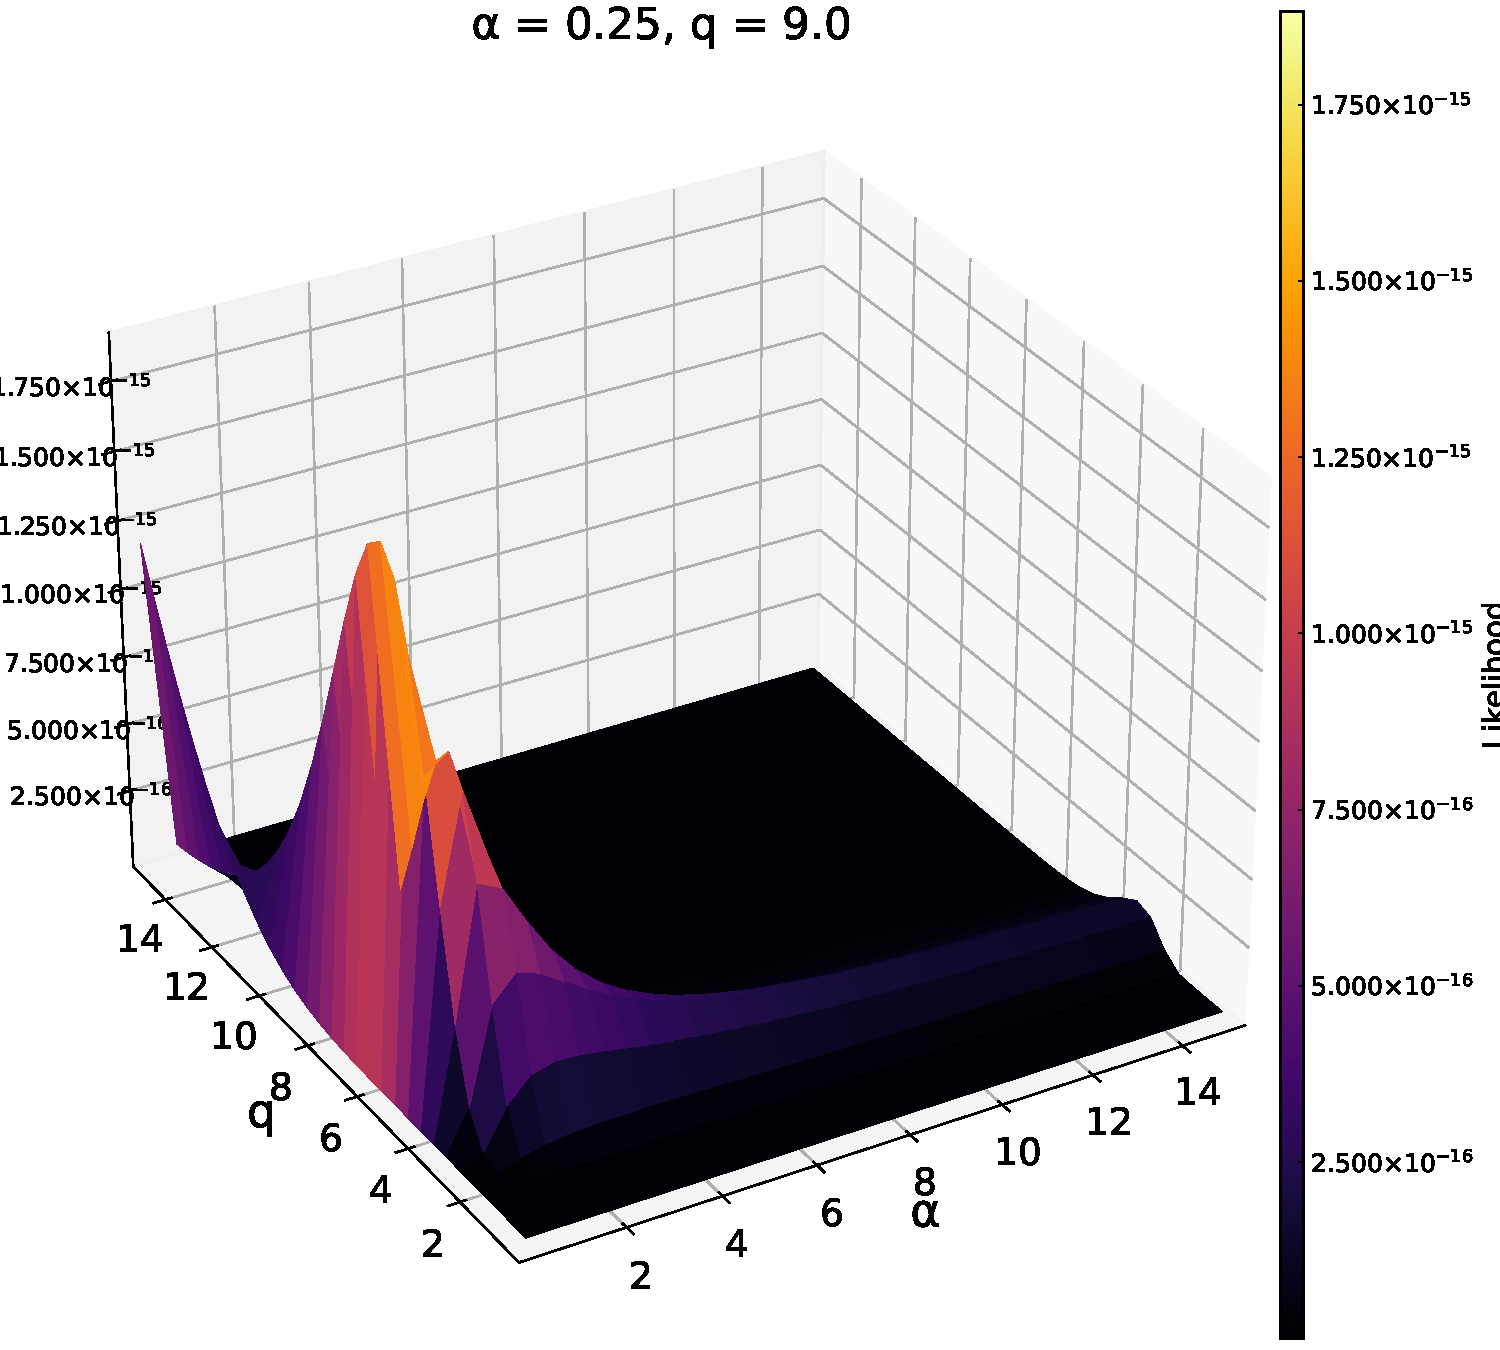
\includegraphics[width=0.9\textwidth]{../figures/Likelihood_sfplt_0.25.pdf} % first figure itself
    \end{minipage}\hfill
    \begin{minipage}{0.45\textwidth}
        \centering
        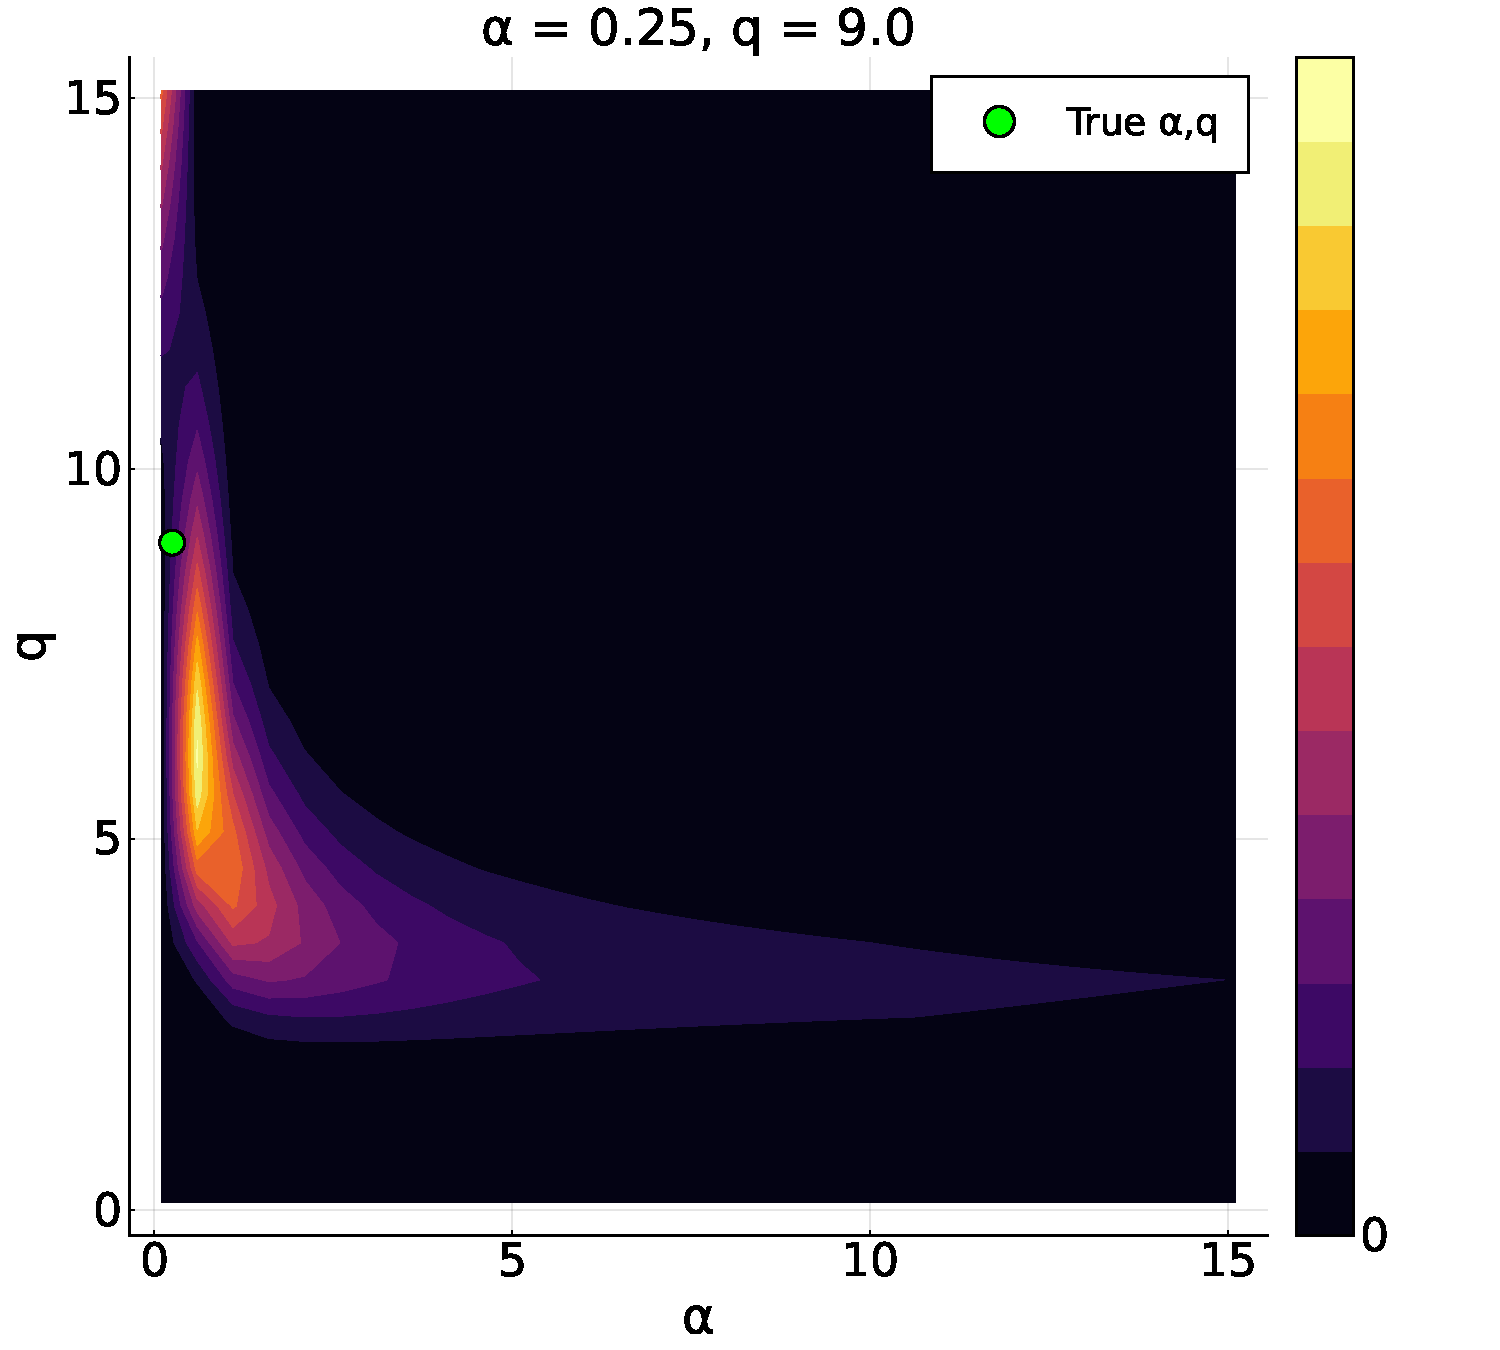
\includegraphics[width=0.9\textwidth]{../figures/Likelihood_contplt_0.25.pdf} % second figure itself
    \end{minipage}
    \caption{\small Likelihood function for data simulated by $\pi \sim Be(0.25, 9 \cdot 0.25), |\mathcal{P}| = 100, n = 10, T = 5$}
\end{figure}

\begin{figure}
    \centering
    \begin{minipage}{0.55\textwidth}
        \centering
        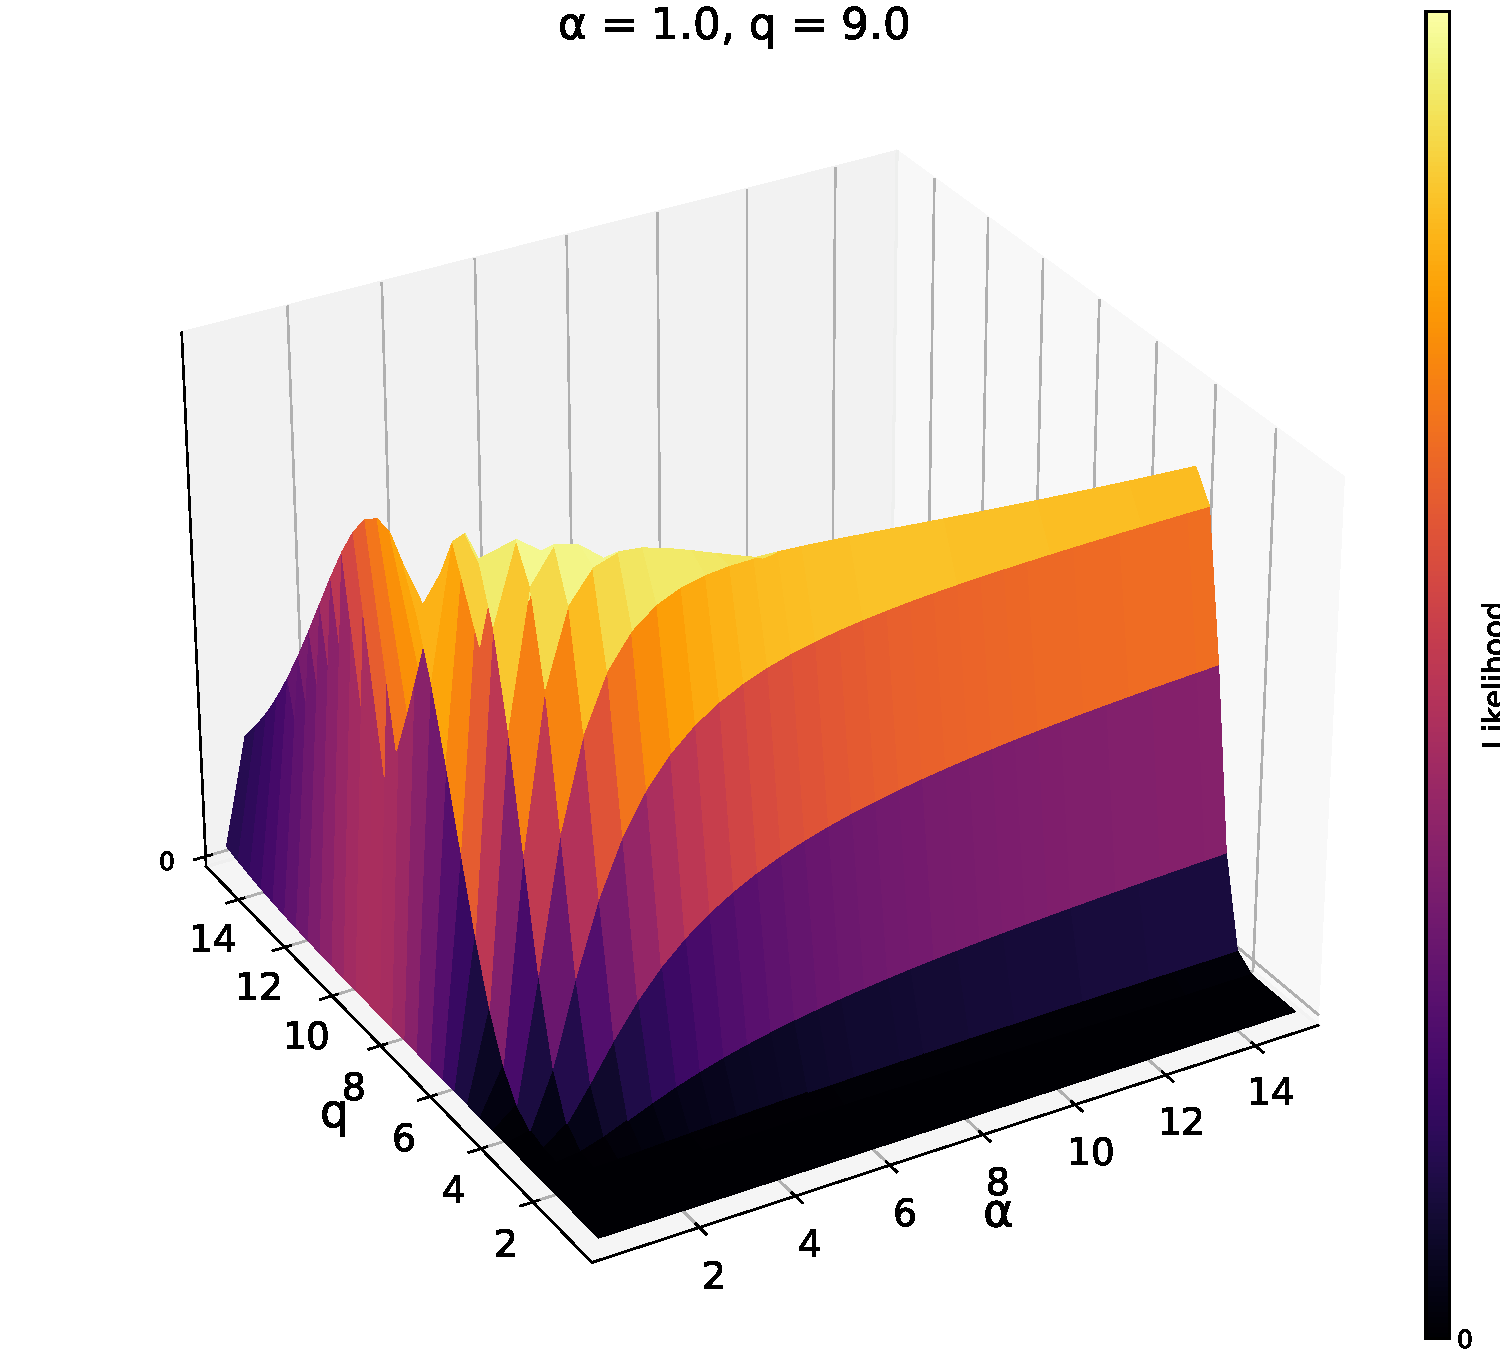
\includegraphics[width=0.9\textwidth]{../figures/Likelihood_sfplt_1.0.pdf} % first figure itself
    \end{minipage}\hfill
    \begin{minipage}{0.45\textwidth}
        \centering
        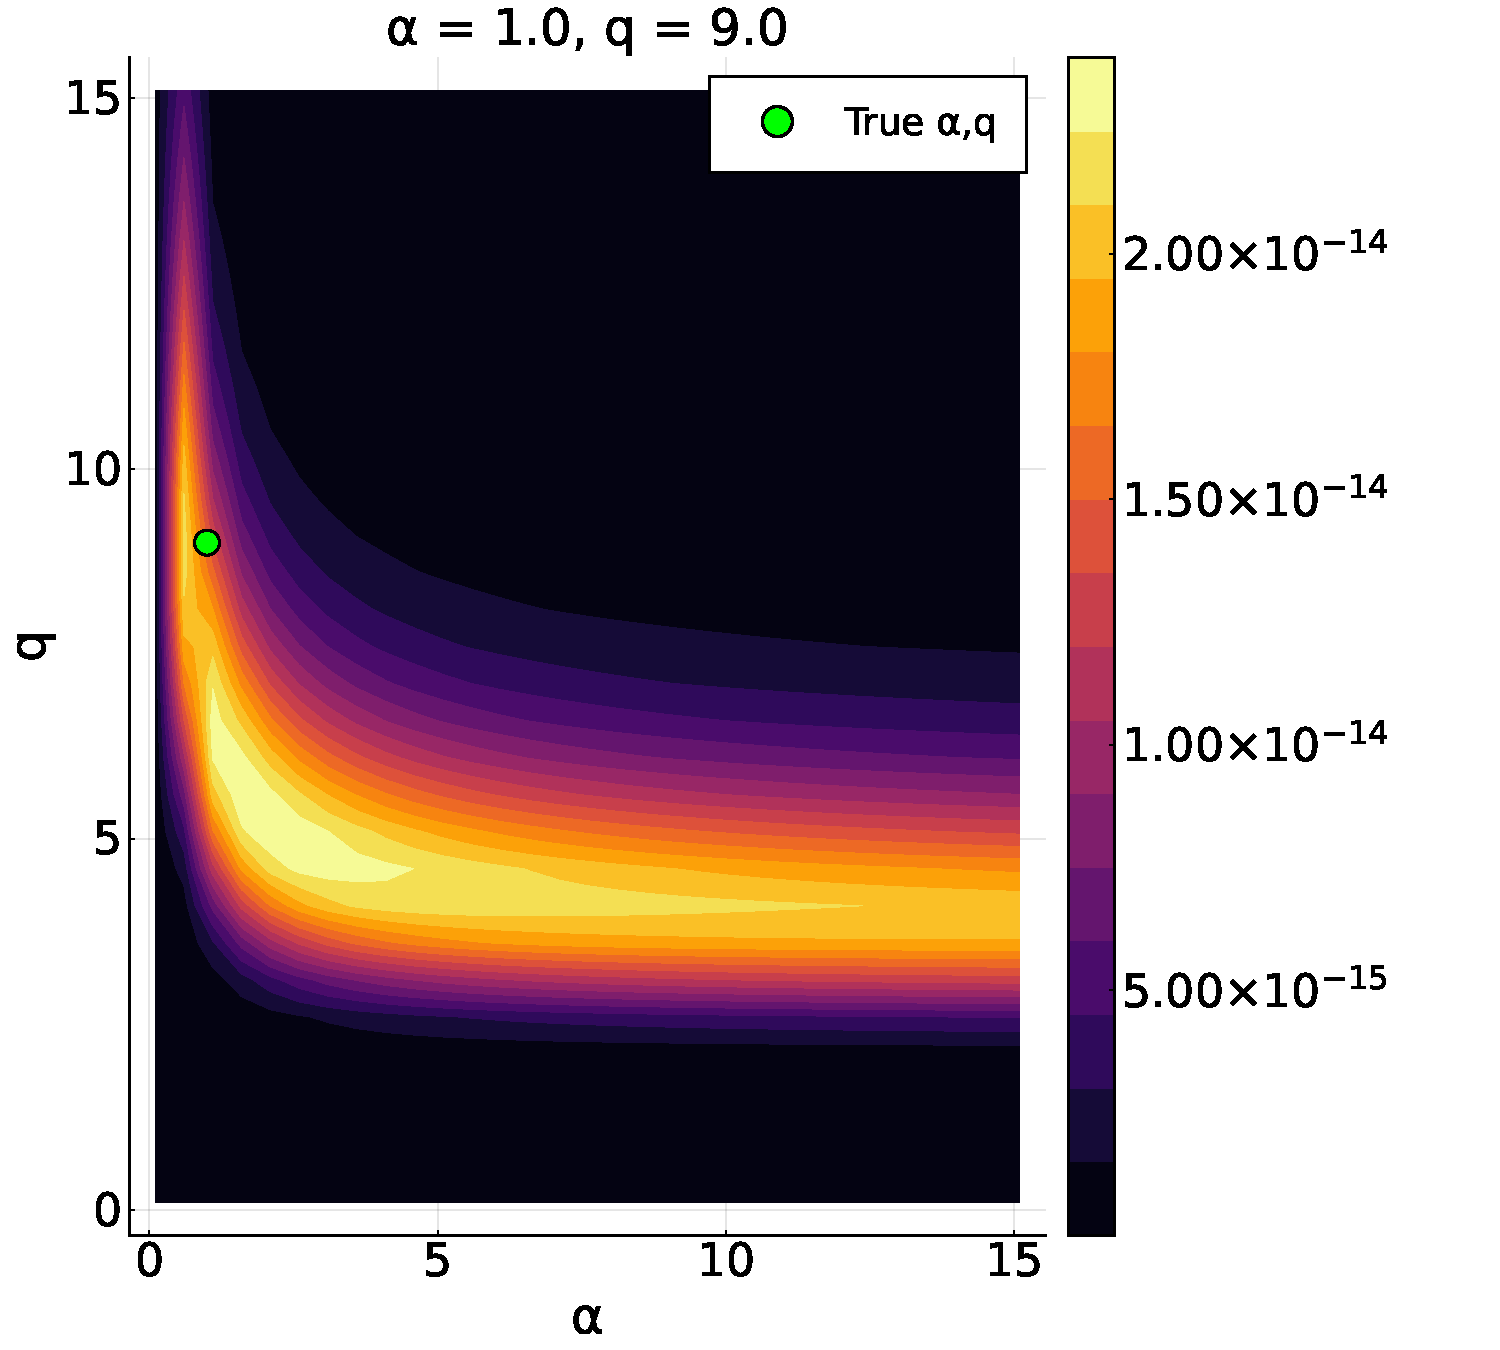
\includegraphics[width=0.9\textwidth]{../figures/Likelihood_contplt_1.0.pdf} % second figure itself
    \end{minipage}
    \caption{\small Likelihood function for data simulated by $\pi \sim Be(1, 9 \cdot 1), |\mathcal{P}| = 100, n = 10, T = 5$}
\end{figure}

\begin{figure}
    \centering
    \begin{minipage}{0.55\textwidth}
        \centering
        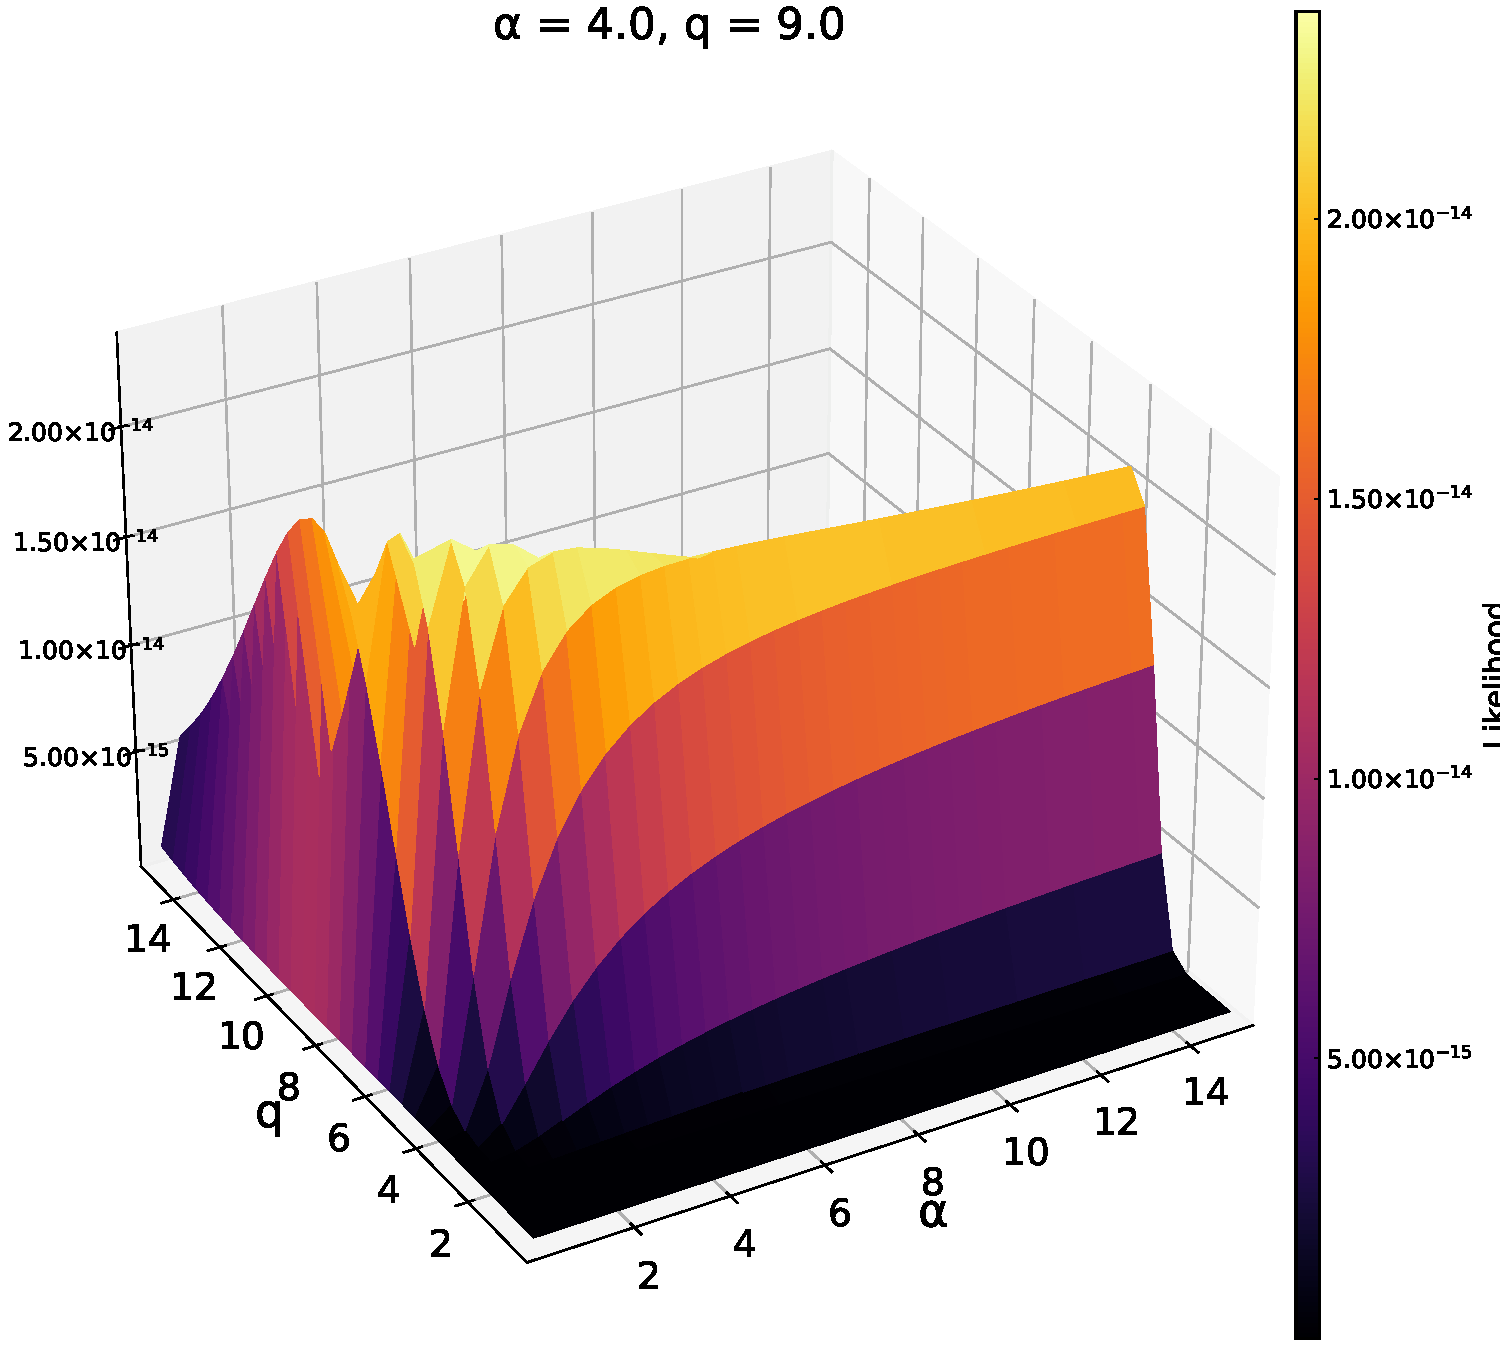
\includegraphics[width=0.9\textwidth]{../figures/Likelihood_sfplt_4.0.pdf} % first figure itself
    \end{minipage}\hfill
    \begin{minipage}{0.45\textwidth}
        \centering
        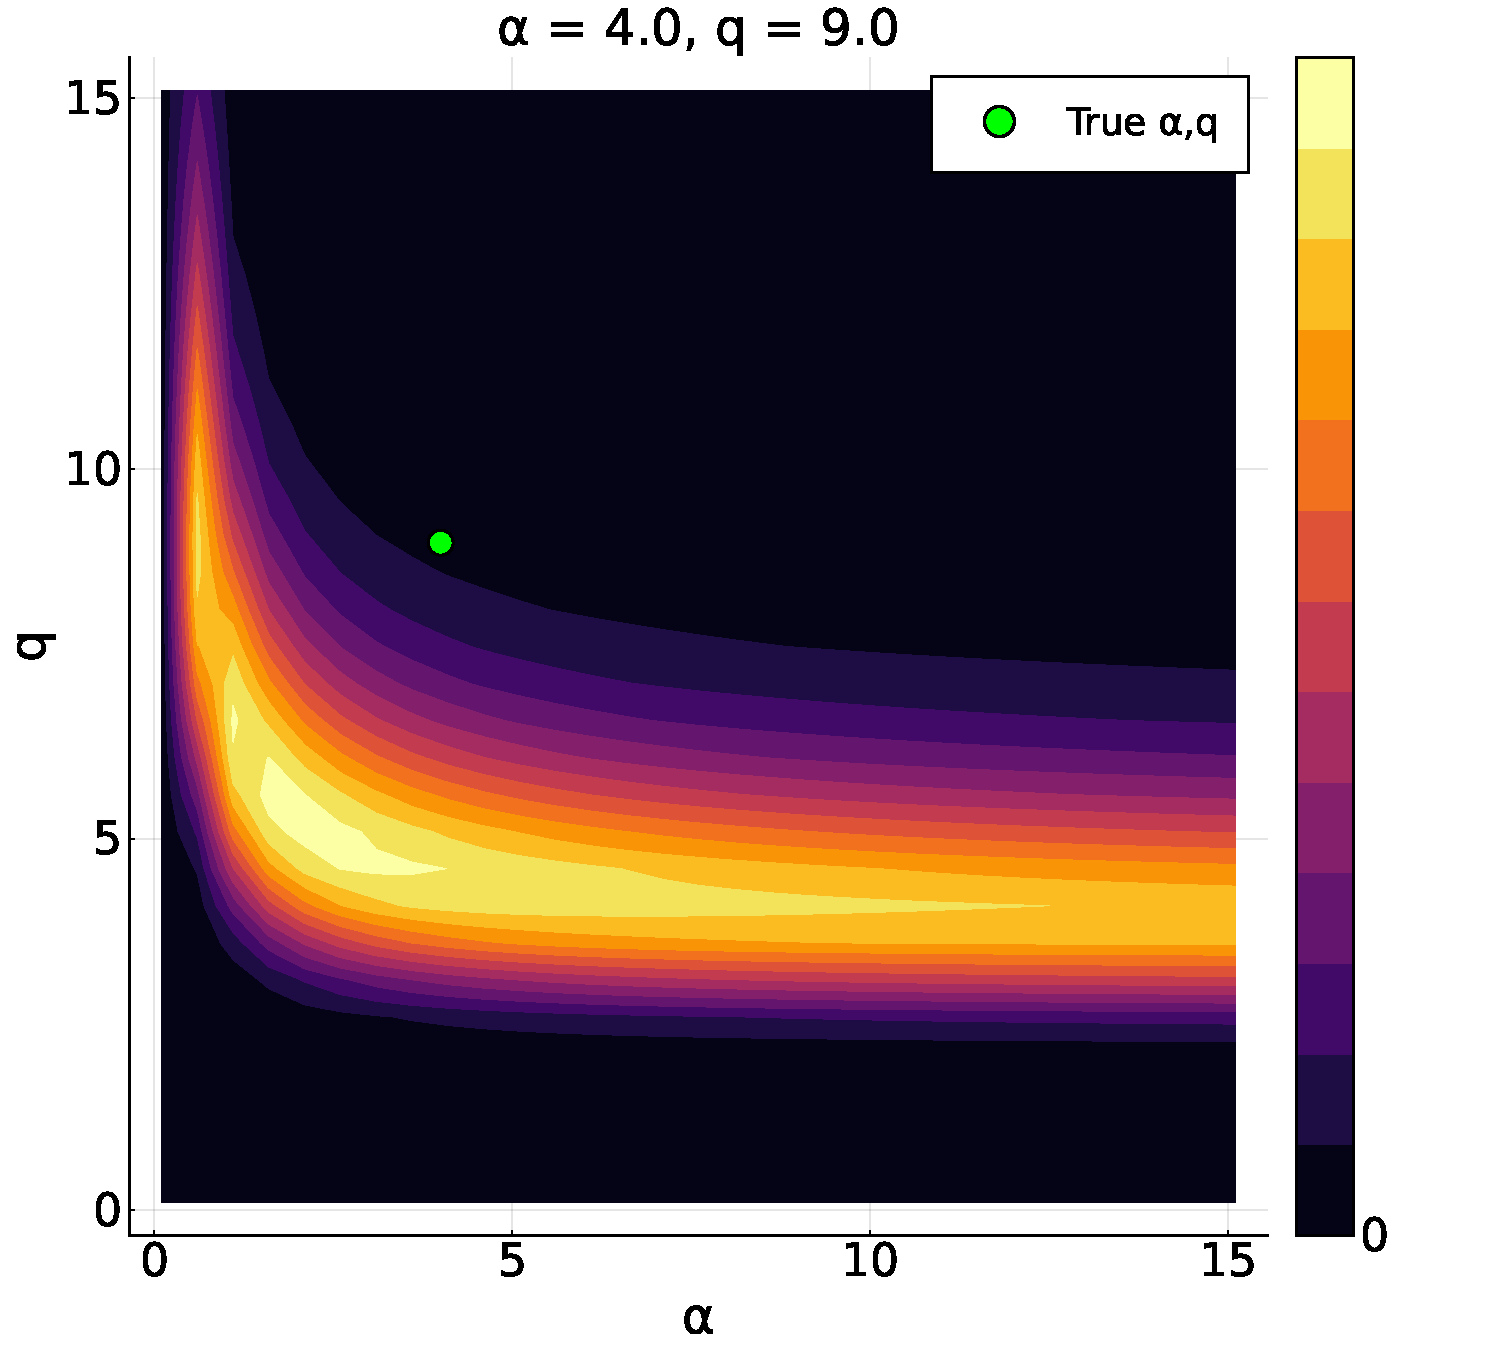
\includegraphics[width=0.9\textwidth]{../figures/Likelihood_contplt_4.0.pdf} % second figure itself
    \end{minipage}
    \caption{\small \small Likelihood function for data simulated by $\pi \sim Be(4, 9 \cdot 4), |\mathcal{P}| = 100, n = 10, T = 5$}
\end{figure}

\end{document}
